\section{Materiais e métodos}
% Estou na dúvida se devo manter os resumos sucintos (como as professoras sugeriram) ou se devo expandi-los mas correr o risco de ou ultrapassar as
% 7 paginas ou de tratar de detalhes secundários e acabar perdendo ponto por isso. Acho que vou esperar para ver a metodologia do Mica para me decidir

\subsection{Extração de DNA}

A extração do DNA genômico foi realizada a partir de amostras biológicas suspeitas de conter 
\textit{Leishmania}, utilizando um protocolo adaptado de Miler, Dykes e Polesky \cite{miller1988salting}. 
O procedimento consistiu em etapas sequenciais de lise celular, ligação do DNA à matriz, lavagens para remoção 
de impurezas e eluição final em tampão PBS, garantindo a obtenção de material genético adequado para análises 
moleculares subsequentes.

\subsection{Espectrofotometria (NanoDrop)}

A quantificação e avaliação da pureza do DNA extraído foram realizadas por espectrofotometria, utilizando o 
equipamento NanoDrop One (Thermo Scientific, EUA). As amostras foram analisadas quanto à concentração (em ng/µL), 
sendo consideradas adequadas aquelas com valores superiores a 100 ng/µL. A razão de absorbância A$_{260}$/A$_{280}$ 
foi utilizada como indicador de contaminação por proteínas, com valores ideais entre 1{,}8 e 2{,}0. Já a razão 
A$_{260}$/A$_{230}$, superior a 1{,}8, indicou baixa presença de contaminantes orgânicos e compostos fenólicos.

\subsection{Reação em Cadeia da Polimerase (PCR)}

A amplificação do DNA foi realizada por meio da Reação em Cadeia da Polimerase (PCR), utilizando primers específicos 
para a detecção do agente etiológico. As condições da reação foram otimizadas para obtenção de um fragmento de tamanho 
previamente determinado. A confirmação da amplificação foi feita por eletroforese em gel de agarose a 1,5\%, corado com 
intercalante de DNA UniSafe (Uniscience), com posterior visualização sob luz ultravioleta

\subsection{Materiais}
\subsubsection{qPCR e High Resolution Melting Analysis}
     
\subsection{Métodos}
\subsubsection{qPCR e High Resolution Melting Analysis}

\begin{wrapfigure}{r}{.45\textwidth}
    \centering
    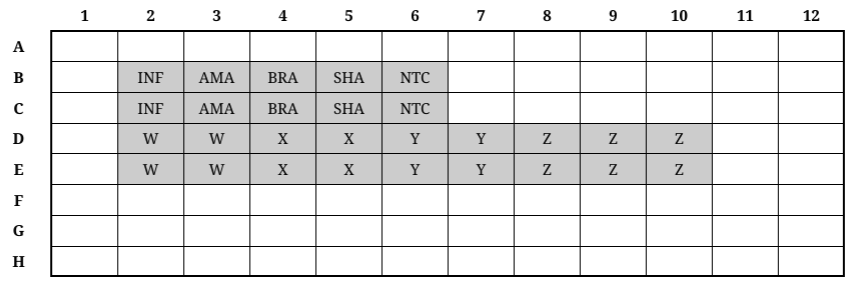
\includegraphics[width=.4\textwidth]{fig/placa_org.png}
    \caption{Disposição das soluções de reação na placa de 96 poços para qPCR. Os poços em branco estão vazios, os poços com solução estão nomeados de acordo com a amostra de DNA. INF - \textit{L. infantum}; AMA - \textit{L. amazonensis}; BRA \textit{L. braziliensis}; SHA - \textit{L. shawi}; NTC - controle negativo; W, X, Y e Z são amostras desconhecidas.}
    \label{wellorg}
\end{wrapfigure}

O protocolo foi adaptado de Zampieri et.al.\cite{HRMzampi2016}.
Foram preparados 28 soluções de \qty{20}{\micro\liter} com
\qty{10}{\micro\liter} de
MeltDoctorTM HRM Master Mix (Thermo fischer Scientific), \qty{0,6}{\micro\liter} de
Primer hsp70-F2, \qty{0,6}{\micro\liter} de Primer hsp70C-R,
\qty{6,3}{\micro\liter} de
água e \qty{2,5}{\micro\liter} de amostra de DNA genômico. Destas 28 soluções,
oito receberam como amostra controle positivo, sendo duas de \textit{L. (L.)
infantum}, duas de \textit{L. (L.) amazonensis}, duas de \textit{L. (V.)
braziliensis} e duas de \textit{L. (V.) shawi}. Duas das soluções receberam
controle negativo, sem DNA genômico. O restante das soluções receberam as
amostras desconhecidas denominadas amostras W, X, Y, Z, sendo quatro soluções de
cada amostra. As soluções foram distribuídas em uma placa de 96 poços conforme a
\cref{wellorg}. A reação de qPCR foi realizada no equipamento StepOne System
(Thermo Fischer Scientific). Primeiro foi feita incubação à \qty{94}{\celsius}
por 5 minutos.  Então, a reação foi submetida à 40 ciclos de desnaturação à
\qty{94}{\celsius} por 30 s, associação e extensão a \qty{60}{\celsius} por 30s. 


